\documentclass[conference]{IEEEtran}



\ifCLASSINFOpdf
\else
\fi



\usepackage{url}
\usepackage{graphicx}
\usepackage{float}
\usepackage{hyperref}
\usepackage[table]{xcolor}
\hyphenation{op-tical net-works semi-conduc-tor}


\begin{document}

\title{Energy-Efficient Smart Buildings by Occupancy
Prediction}


% author names and affiliations
% use a multiple column layout for up to three different
% affiliations
\author{\IEEEauthorblockN{Mina Moghaddam}
\IEEEauthorblockA{Dept. of Computer Engineering\\
		     Middle East Technical University\\
			Ankara, Turkey\\
			Mina.moghaddam90@gmail.com}
\and
\IEEEauthorblockN{Tahsincan K{\"o}se}
\IEEEauthorblockA{Dept. of Computer Engineering\\
		     Middle East Technical University\\
			Ankara, Turkey\\
			tahsincan.kose@ceng.metu.edu.tr}
\and
\IEEEauthorblockN{M. Ra\c{s}it {\"O}zdemir\\}
\IEEEauthorblockA{Dept. of Computer Engineering\\
		     Middle East Technical University\\
			Ankara, Turkey\\
			rasit.ozdemir@metu.edu.tr}
\and
\IEEEauthorblockN{\ \ \ \ \ \ \ \ \ }
\IEEEauthorblockA{\ \ \ \ \ \ \ \ \ }
\and

\IEEEauthorblockN{\hspace{3.5cm}Zakiah Utami}
\IEEEauthorblockA{\hspace{3.5cm}Dept. of Computer Engineering\\
		     \hspace{3.5cm}Middle East Technical University\\
			\hspace{3.5cm}Ankara, Turkey\\
		    \hspace{3.5cm}utami.zakiah@metu.edu.tr}
\and
\IEEEauthorblockN{\hspace{-2cm}Seyda Ertekin}
\IEEEauthorblockA{\hspace{-2cm}Dept. of Computer Engineering\\
		     \hspace{-2cm}Middle East Technical University\\
			\hspace{-2cm}Ankara, Turkey\\
		    \hspace{-2cm}seyda@ceng.metu.edu.tr}
}




% make the title area
\maketitle

% As a general rule, do not put math, special symbols or citations
% in the abstract
\begin{abstract}
Based on the increase in energy
consumption, energy efficiency has become a
paramount topic. Through the energy conservation
studies, it can be achieved by predicting occupant
presence in buildings. In this study, the accuracy of
occupancy prediction has been tested on data from
differences in levels of Light, CO2, and Humidity in
intervals of 1, 3, and 5 minutes. Artificial Neural
Networks (ANN), Support Vector Machines (SVM), and
Decision Trees have been chosen as learning
algorithms. Various setups and hyper-parameters are
used and the accuracy is in range of 80 to 90 percent.
The study shows that using data generated from only
changes in values of parameters, despite being more
general than absolute values, have still a high prediction
accuracy.\\

Index Terms --- Building energy efficiency, machine
learning, occupancy prediction, office room.
\end{abstract}



\section{Introduction}
In this era, occupation in human spaces impress
different aspects of a building like light, temperature,
humidity and so on. It is of little debate in today’s world
that modeling occupant behavior and its information is of
great importance. It is quite expected to notice significant
energy savings that can be achieved by the accurate
prediction of occupancy in buildings. In this developed
society, commercial office buildings require a large
amount of area and energy to create a comfort zone for
their occupants\cite{OccMeasure}. With this in mind, the office buildings are useful targets for modeling occupant behavior to manage its potential of energy sources accurately in order to increase energy savings. In a recent study, it is illustrated that accurate occupation prediction in buildings has been estimated at 15 to 25 \% energy savings\cite{ReductoHVAC}. In another simulation-based study\cite{SensorOcc}, the potential energy savings is suggested as approximately 30\%.\\

Current status
of industrial energy consumption possesses an important
risk to society and environment in terms of sufficiency of
resources. Although various governments around the
globe have set quantified targets that anticipate 20\%\cite{TargetCons} energy usage reduction in overall, the total industrial consumption still follows an ascending trend. Also, commercial office buildings comprise the majority of in-
floor areas in most of the developed countries hence consume the remarkable amount of energy in the logistics of building services. Having all these considered the problem with regards to the necessity of effective energy usage. Meanwhile, this implies the minimization of resource dissipation in such enormous in-floor areas. In fact, this is just a single part of the whole problem. Thinking on a global scope brings one to the problem of world's inability to restore its natural resources fully anymore. Failing to capture this problem would result in higher energy wastage which becomes more and more profoundly threatening for the entire world. For that reason, resolving this sub-problem would effectively
inspire all other sectors, thus affects the whole problem in long-term.

\section{Method}
This paper aims to predict occupation in an office room during different hours based on the data from light, temperature, humidity and CO2 by using Machine Learning approach. There were used three datasets for training and testing, that two testing datasets for open and close door in the office \cite{Candanedo}.\\


The original article in which the dataset was gathered and analyzed used a variety of statistical approaches on
the data. Our aim is to take ANN, SVM\cite{Erickson} and Decision Tree methods to increase the accuracy in a generalized version of the problem, which we believe that is a more extensive solution regarding to the overall problem.

The datasets consist of labeled training and test data with 7 attributes: Time, Temperature, Relative Humidity, Light, CO2, Humidity Ratio, and Occupancy. Training data consists of 8143 entities. Test data is divided into two portions, one is data gathered while the door was closed, with 2665 rows of data, and the other one is data gathered while the door was open, with 9752 rows of data \cite{Ryu}.

We have used the already existing information to augment the data with 9 new attributes. These 9 new attributes are: Differences of CO2/Humidity and Light level in 1,3 and 5 minutes of intervals respectively. We embrace this approach to globalize the model. The previous study \cite{Pedersen} have used absolute values which can be attributed to a certain location or time. By training a model using only the differences of features, we are assuming the model would become more invariant to time and location.


\section{Evaluation}
Before anything, it is highly beneficial to make descriptive analysis on the data rather than throwing it into models. For this purpose, visualizing data is a good first practice. Recalling that the dataset is processed, it now constitutes of 9 attributes which require a hyperplane representation. In order to have a decent visualization, reducing the parameter space to 2 and 3 most important ones (only for visualization) using \textit{Feature Selection}\cite{Guyon} is a common method. However, feature selection might not provide a clear separation between the distinct classes. Such a separation heavily depends on the complexity of data. \textit{\textbf{sklearn}} library is used throughout the model setups in the course of feature manipulation tasks in which all these are readily implemented to facilitate one-line usages. For instance, \textbf{K} best features in terms of \textit{\textbf{chi square}}\cite{Fahim} independence (relatedness) score metrics are extracted through utilization of aforementioned library. All in all, best features are plotted in a scattered manner to gain a deeper understanding on the dataset. Nonetheless, we couldn't achieve a clear separation between the classes. Corresponding figure represent the best resulting layouts that have the highest visual separations.

\begin{figure}[H]
	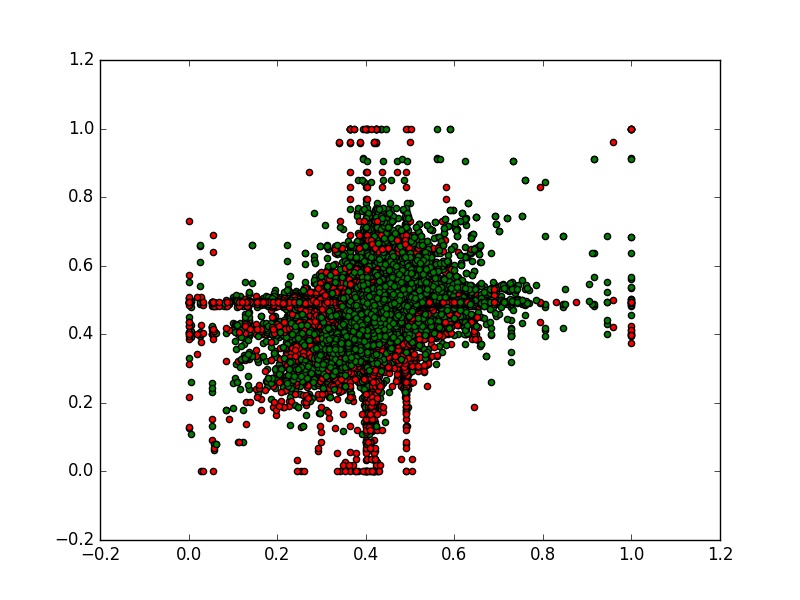
\includegraphics[width=1\columnwidth]{best_2features.jpg}
	\caption{Visualization with 2 Best Features}
	\label{2plot}
\end{figure}

Lastly, the training data is composed of 1729 positive instances (occupied) whereas 6414 ones are negative instances (non-occupied). This is a slightly imbalanced dataset, thus considering accuracy would not be a bad choice. Also as a supporting performance metrics, \textit{F1 score} possesses a complementary role. Having all these considered, we have trained several ANNs, SVMs and Decision Trees with different sets of hyper-parameters to compare the estimation rates.

\vspace{-0.1cm}

\subsection{Artificial Neural Network}

Our hypothesis states that it is possible to predict occupancy in a space with only using differences in Light level, CO2 level and Humidity level. In order to test the hypothesis, several configurations are constructed to find the optimum model.\\

In the beginning, a neural network is constructed to initiate experimentation with 2 hidden layers having 10 and 8 hidden units respectively. Input layer contains  9 input units by the number of attributes, whereas output layer contains 2 output units. Learning rate is determined as $\alpha = 0.001$. Loss criterion is \textit{cross entropy} and optimizer function is chosen as \textit{Adam} optimizer\cite{Adam}. \textit{Sigmoid} function is the activation function in all layers except the output layer. Output layer employs \textit{softmax} activation function.

As it is seen in the Figure \ref{mix_lr}, loss number reaches a local minima at generally 1500 epoches. Since Adam is a variation of Stochastic Gradient Descent, loss does not stabilize and starts producing tiny fluctuations. Stochastic Gradient Descent methods have the ability to recover from local minimum and that is the underlying reason for this phenomenon. Its rate is determined by the nearly extinguished gradients. Therefore, learning process is in proximity of an equilibrium state. Continuing loss reduction only contributes to over-fitting, so learning with high number of epochs will not pay off.


\begin{figure}[H]
	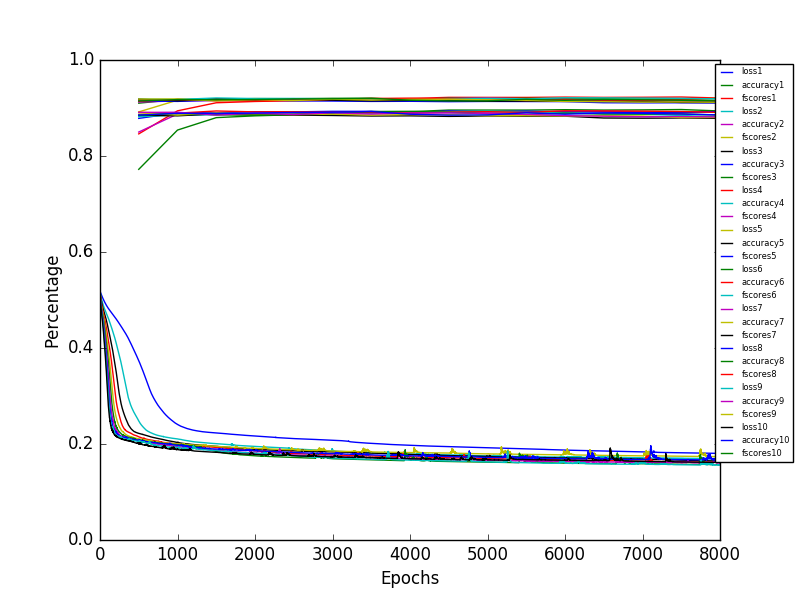
\includegraphics[width=0.9\columnwidth]{mix_plot_lr.png}
	\caption{Loss, Accuracy, F1 Score of $\alpha \in [0.001 - 0.01]$ with step 0.001} 
	\label{mix_lr}
\end{figure}

Figure \ref{mix_lr} graphs loss,  accuracy, F1 score values with respect to learning rates and epochs based on a grid-search approach. \textit{loss1} denotes the loss curve with learning rate 0.001. All subsequent curves are plotted in this manner, i.e. index on right-hand side is multiplied by a factor of 0.001. This set of experiments output \textit{accuracy} and \textit{F1 score} with learning rate $\alpha=0.009$ at epoch 2500 as at most \textbf{0.8961} and \textbf{0.9221} respectively. A very brief and concise comment can be brought about the figure above; that is, as learning rate increases the speed of loss convergence and fluctuations increase, which makes them \textit{relatively bad} models especially with higher number of epochs.\\

Experiments thus far have been done with a simple model. Architecture adjustment is normally required when there are over-fitting or under-fitting issues in the learning process. Nonetheless, this model does not suffer from those two; thus, adjusting the number of layers and their sizes would not make any significant improvements on the estimations. In any case, this assumption should be tested via experimentation on these particular hyper-parameters. Note that learning rate is fixed to 0.009.\\

\begin{table}[H]
	\centering
	\caption{Epoch vs. Accuracy of Several Architectures - Closed Door}
	\label{AllArches}
	\begin{tabular}{|l|l|l|l|l|l|}
		\hline
		& \textit{9x10x10x8x4} 
		& \textit{9x16x8x8x4}
		& \textit{9x10x8x12x4 \textbf{*}}
		& \textit{9}
		& \textit{9x8}\\ \hline
		\textbf{500} & 0.893 & 0.890 & 0.884 & 0.820 & 0.879\\ \hline
		\textbf{1000} & \cellcolor{green!25}0.898 & 0.890 & 0.893 & 0.820 & 0.891\\
		\hline
		\textbf{1500} & 0.894 & 0.886 & 0.896 & 0.820 & 0.892\\ \hline
		\textbf{2000} & 0.892& 0.883 & 0.894 & 0.820 & 0.889\\ \hline
		\textbf{2500} & 0.892 & 0.878 & 0.890 &  0.821 & 0.601\\
		\hline
		\textbf{3000} & 0.894 & 0.879 & 0.887 & 0.821 & 0.878\\ \hline
		\textbf{3500} & 0.894 & 0.878 & 0.888 & 0.821 & 0.885\\ \hline
		\textbf{4000} & 0.890 & 0.875 & 0.885 & 0.821 & 0.880\\ \hline
		\textbf{4500} & 0.893 & 0.874 & 0.886 & 0.821 & 0.880\\ \hline
		\textbf{5000} & 0.893 &  0.872 & 0.885 & 0.821 & 0.883\\ \hline
	\end{tabular}
\end{table}
\indent\textbf{*} Hidden layer before the output layer utilizes \textit{ReLU} activation function instead of sigmoid.\\

Except the linear model, all models roughly perform the same as can be seen in the figure. After several experiments, first architecture with 4 hidden layers with respectively 10, 10, 8 and 4 hidden units outputs the best accuracy of \textbf{0.898} at 1000 epochs among other configurations. Reaching such an accuracy rate in shorter training durations is also another advantage.\\

Above experiments serve the base for fine-tuning for overall model to improve and thus only consider first test set which is gathered when the door is closed. A similar table to Table \ref{AllArches} is sketched below for open door test set.\\

Note that, initial architecture which employs different loss criteria and an additional dropout computed  substantially less accuracy rates for open door dataset. This is simply because of the increasing noise in the sensor data when the door is opened.

\begin{table}[H]
	\centering
	\caption{Epoch vs. Accuracy of Several Architectures - Opened Door}
	\label{AllArches2}
	\begin{tabular}{|l|l|l|l|l|l|}
		\hline
		& \textit{9x10x10x8x4} 
		& \textit{9x16x8x8x4}
		& \textit{9x10x8x12x4 \textbf{*}}
		& \textit{9}
		& \textit{9x8}\\ \hline
		\textbf{500} & 0.778 & 0.795 & 0.789 & 0.789 & 0.790\\ \hline
		\textbf{1000} & 0.804 & 0.805 & 0.799 & 0.789 & 0.797\\
		\hline
		\textbf{1500} & 0.808 & 0.812 & 0.790 & 0.789 & 0.810\\ \hline
		\textbf{2000} & 0.807& 0.810 & 0.794 & 0.789 & \cellcolor{green!25}0.815\\ \hline
		\textbf{2500} & 0.807 & 0.812 & 0.803 &  0.786 & 0.814\\
		\hline
		\textbf{3000} & 0.804 & 0.810 & 0.801 & 0.789 & 0.814\\ \hline
		\textbf{3500} & 0.802 & 0.807 & 0.799 & 0.787 & 0.808\\ \hline
		\textbf{4000} & 0.801 & 0.804 & 0.798 & 0.786 & 0.803\\ \hline
		\textbf{4500} & 0.798 & 0.801 & 0.798 & 0.785 & 0.803\\ \hline
		\textbf{5000} & 0.793 &  0.798 & 0.797 & 0.785 & 0.800\\ \hline
	\end{tabular}
\end{table}

In this set of experiments, last architecture reaches to the best accuracy of \textbf{0.815 }rate among others as can be seen in Table \ref{AllArches2}. Learning rate $\alpha$ is fixed to 0.009 as in the first set of experiments.\\

The high accuracy in these tests proves that it is possible to use
this augmented data to predict occupancy of an environment. In order to compare approaches and find better, if any, models, we proceed with SVMs and Decision Trees.

\subsection{Suport Vector Machines}
For Support Vector Machine method, we configure the SVM parameters and report their results. We record the results for two performance metrics: accuracy and F1 score.\\

We tried a number of configurations in terms of hyperparameters such as penalty parameter(C), tolerance for stopping criterion, kernel function and gamma(kernel coefficient for kernel functions) while constructing Support Vector Machine models. Since SVM results are not good enough as the other methods, we lay out only the maximum results we get during the experiments and provide the link to the results of all other configurations for the ones who aspire to inspect in greater detail. Best accuracy and F1 score are 0.864520 and 0.798351 respectively with the model \textbf{(C=0.327, tol=0.0136,gamma='auto',kernel='rbf')} for closed door test set. We have made coarse and grid searches to find out the best performing Support Vector Machine \textbf{(C=0.2375, tol=0.0,gamma=2.8',kernel='rbf')} for open door test set. Although we got quite a good accuracy of 0.811833, F1 score is merely 0.599711.

\subsection{Decision Trees}
The main idea behind the decision tree algorithm is to build a tree-like model from root to leaf nodes. All nodes receive a list of inputs and the root node receives all the examples in the training set. Each node asks a true or false question for a feature and responses by partitioning into two subsets. The subsets then become the input the child nodes where the child node asks another question for one of the other features.\\

Below are the tables consisting of the experimental data from two cases, closed and open door. In sci-kit learn library, we can configure "Max Samples Split" and "Max Samples Leaf" parameters as floating-point numbers, then they will be percentages that implies the minimum number of samples for each node.

\begin{table}[H]
	\centering
	\caption{Accuracy and F1-Score of Closed Door Case}
	\label{AllArches5}
	\begin{tabular}{|p{1cm}|p{0.7cm}|p{0.7cm}|p{0.7cm}|p{1cm}|p{1cm}|p{1cm}|p{1cm}|}
	    \hline
		\textit{Criterion} 
		& \textit{Max Depth}
		& \textit{Min Samples Split}
		& \textit{Max Features}
		& \textit{Min Samples Leaf}
		& \textit{Accuracy}
		& \textit{F1 Score}\\ \hline
		gini & 6 & 2 & log2 & 1 & 0.8923 & 0.8782\\ \hline
		gini & 2 & 2 & log2 & 1 & 0.9062 & 0.8961\\ \hline
		gini & None & 0.3 & log2 & 1 & 0.9362 & 0.9311\\ \hline
		gini & None & 0.5 & log2 & 1 & 0.9358 & 0.9305\\ \hline
		gini & None & 0.8 & log2 & 1 & 0.9062 & 0.8961\\ \hline
		gini & None & 0.25 & log2 & 1 & 0.9358 & 0.9305\\ \hline
		gini & None & 0.35 & log2 & 1 & \cellcolor{green!25}0.9366 & \cellcolor{green!25}0.9314\\ \hline
		entropy & None & 0.35 & auto & 1 & 0.9354 & 0.9301\\ \hline
		entropy & None & 0.35 & auto & 0.01 & 0.9305 & 0.9247\\ \hline
	\end{tabular}
\end{table}

As we can see from the table above, we started the experiment by comparing the Criterion function. We got the accuracy better when we use gini index instead of entropy gain. Focusing on gini index, we iterate to find the best number of the maximum depth of the tree, and find "None" is the best on this case. Then we tune the Min Samples Split hyperparameter. The best value for the test data is 0.35. Min Samples Split parameter plays a key role in this experiment, because it eliminates overfitting. We then try some possible values for Max Features and Max Samples Leaf. As the result, the maximum \textit{accuracy} after training for the case of closed door is \textbf{0.9366} with \textit{F1 score} is \textbf{0.9314}, when gini criteria was used for the Gini impurity and the minimum number of samples required to split an internal node is 35\%. \\


\begin{table}[H]
	\centering
	\caption{Accuracy and F1-Score of Open Door Case}
	\label{AllArches7}
	\begin{tabular}{|p{1cm}|p{0.7cm}|p{0.7cm}|p{0.7cm}|p{1cm}|p{1cm}|p{1cm}|p{1cm}|}
	    \hline
		\textit{Criterion} 
		& \textit{Max Depth}
		& \textit{Min Samples Split}
		& \textit{Max Features}
		& \textit{Min Samples Leaf}
		& \textit{Accuracy}
		& \textit{F1 Score}\\ \hline
		gini & 6 & 2 & log2 & 1 & \cellcolor{green!25}0.8513 & \cellcolor{green!25}0.7587\\ \hline
		entropy & 6 & 2 & log2 & 1 & 0.8481 & 0.7335\\ \hline
		gini & None & 2 & log2 & 1 & 0.8114 & 0.7306\\ \hline
		gini & 3 & 2 & log2 & 1 & 0.8409 & 0.6851\\ \hline
		gini & 2 & 2 & log2 & 1 & 0.8111 & 0.6846\\ \hline
		gini & 10 & 2 & auto & 1 & 0.8399 & 0.7425\\ \hline
		gini & 8 & 2 & auto & 1 & 0.8465 & 0.7548\\ \hline
		gini & 5 & 2 & auto & 1 & 0.8477 & 0.7368\\ \hline
		gini & 5 & 0.02 & auto & 1 & 0.8459 & 0.7502\\ \hline
	\end{tabular}
\end{table}

While in experiment of the open door case as shown in table above, by doing similar approach as done in previous case, the best \textit{accuracy} obtained is \textbf{0.8513} with \textit{F1 score} is \textbf{0.7587} when we use gini criterion with maximum depth is 6 and the number of maximum features is the log2 of the number of the features.\\

More, by comparing the "Max Feature" values, we also see that the best accuracy is always obtained when the number of maximum features to consider when looking for the best split is set to be log2 for this dataset. \\

\section{Conclusion}
The main purpose of this research is to test different
machine learning methods which can successfully predict
occupancy status of an environment using the generalized
version of data from \cite{Candanedo}. Some of the crucial factors
present in the original data which can give a very high
predictive power, such as time of the day, is completely
omitted from the data set in favor of generalization. The
remaining factors have been processed for new attributes.
Our hypothesis was, given a good model, Decision Trees and Artificial
Neural Networks can reach a reliable accuracy. Our research result, which is present
in the Evaluation section of the article shows that both Decision Trees and ANN have the capability of reaching up to 90
percent accuracy. We included prediction results of
Support Vector Machines to compare with the original article.\\

Overall, despite that original authors have cast side Decision Trees and
Artificial Neural Networks for not being accurate enough, the result of this research confirms that using generalized data to train Decision Trees and Artificial
Neural Networks can reach a fair accuracy even without using time or other absolute
attributes.


\begin{thebibliography}{1}
\bibitem{OccMeasure}
T. Labeodan, et al, \emph{\textbf{Occupancy   measurement   in   commercial   office  
buildings   for   demand-driven   control   applications   -   A   survey   and   detection   system   evaluation.}}\\  
Journal of Energy and Buildings. 93(2015), pp. 303-314.
\bibitem{ReductoHVAC}
V. L. Erickson, et al,    \emph{\textbf{OBSERVE: Occupancy-based system for efficient reduction of HVAC energy.}}\\Proceedings   of   the   10th   ACM/IEEE   International   Conference  
on Information Processing in Sensor Networks, 258-269 (2011).
\bibitem{SensorOcc}
B.   Dong,   B.   Andrews, \emph{\textbf{Sensor-based   Occupancy   Behavioral   Pattern   Recognition   For   Energy  
And   Comfort   Management   In   Intelligent   Buildings}}\\Eleventh   International   IBPSA   Conference,  
1444-1451 (2009).
\bibitem{TargetCons}
E.U, \emph{\textbf{Directive 2010/31/EU of the European Parliament and of the Council of 19
May 2010 on the Energy Performance of Buildings (Recast)}}, Official Journal of the
European Union, vol. 18, no. 6, pp.13–33, 2010.
\bibitem{Candanedo}
L. M. Candanedo, V. Feldheim, \emph{\textbf{Accurate occupancy detection of an office room from light, temperature, humidity and CO2 measurements using statistical learning models}}, Energy and Buildings. 112, (2016) 28-39.
\bibitem{Erickson}
V. L. Erickson, M. Á. Carreira-Perpiñán, A. E. Cerpa, \emph{\textbf{Occupancy Modeling and Prediction for Building Energy Management.}} ACM Transactions on Sensor Networks. 10, 1-28 (2014).
\bibitem{Ryu}
S. H. Ryu, H. J. Moon, \emph{\textbf{Development of an occupancy prediction model using indoor environmental data based on machine learning techniques.}} Building and Environment. 107, 1-9 (2016).
\bibitem{Pedersen}
T. H. Pedersen, K. U. Nielsen, S. Petersen, \emph{\textbf{Method for room occupancy detection based on trajectory of indoor climate sensor data.}} Building and Environment. 115, 147-156 (2017).
\bibitem{Guyon}
I. Guyon, A. Elisseeff  \emph{\textbf{An Introduction to Variable and Feature Selection}}
Journal of Machine Learning Research 3  1157-1182 (2003).
\bibitem{Fahim}
M. F. Zibran
\emph{\textbf{CHI-Squared Test of Independence}}
\bibitem{Adam}
D. P. Kingma, J. L. Ba
\emph{\textbf{Adam: A Method for Stochastic Optimization }}
International Conference on Learning Representations (2015).
\end{thebibliography}




% that's all folks
\end{document}


